\documentclass[svgnames]{beamer}
\usepackage{etex}
\reserveinserts{28}
\usetheme[pageofpages=of,% String used between the current page and the
                         % total page count.
          titleline=true,
          alternativetitlepage=true,% Use the fancy title page.
          titlepagelogo=figures/LSU-logo-small,% Logo for the first page.
          watermark=figures/LSU-logo-small
          ]{Torino}
%\usecolortheme{stellar}
\usepackage{listings}
\ifxetex
\usepackage{fontspec}
\defaultfontfeatures{Mapping=tex-text}
\setsansfont[Path = fonts/,ItalicFont={gillsansmtpro-bookitalic-opentype.otf}]{gillsansmtpro-book-opentype.otf}
\setmonofont[Path = fonts/]{inconsolata-opentype.otf}
\newcommand{\codefont}{\ttfamily}
\else
\usepackage[utf8x]{inputenc}
\usepackage[nott]{inconsolata}
\newcommand{\codefont}{\fontfamily{fi4}\selectfont}
\fi
\usepackage{color}
\usepackage{xcolor}
\usepackage[english]{babel}
\usepackage{verbatim}
\usepackage{tikz}
\usepackage{graphicx}
\graphicspath{{./figures/}}
\usetheme{metropolis}

\definecolor{dkgreen}{rgb}{0,0.6,0}
\definecolor{lsupurple}{RGB}{70,29,124}
\definecolor{lightlsupurple}{RGB}{102,46,145}
\definecolor{lsugold}{RGB}{253,208,35}
\definecolor{lsugray}{RGB}{153,153,153}
\definecolor{darkgold}{RGB}{210,159,19}
\definecolor{brown-web}{rgb}{0.65,0.16,0.16}

\title{Extending Distributed Functionality in Phylanx}
\author{Maxwell Reeser}
\institute{Louisiana State University \\ Center for Computation and Technology \\
The STEllAR Group}
\date{November 7, 2019}

\begin{document}
\makeatletter
\newenvironment{btHighlight}[1][]
{\begingroup\tikzset{bt@Highlight@par/.style={#1}}\begin{lrbox}{\@tempboxa}}
{\end{lrbox}\bt@HL@box[bt@Highlight@par]{\@tempboxa}\endgroup}

\newcommand\btHL[1][]{%
  \begin{btHighlight}[#1]\bgroup\aftergroup\bt@HL@endenv%
}
\def\bt@HL@endenv{%
  \end{btHighlight}%
  \egroup
}
\newcommand{\bt@HL@box}[2][]{%
  \tikz[#1]{%
    \pgfpathrectangle{\pgfpoint{1pt}{0pt}}{\pgfpoint{\wd #2}{\ht #2}}%
    \pgfusepath{use as bounding box}%
    \node[anchor=base west, fill=orange!30,outer sep=0pt,inner xsep=1pt, inner ysep=0pt, rounded corners=3pt, minimum height=\ht\strutbox+1pt,#1]{\raisebox{1pt}{\strut}\strut\usebox{#2}};
  }%
}
\makeatother

\lstset{ %
  language=C++,                   % the language of the code
  basicstyle=\ttfamily\scriptsize,% the size of the fonts that are used for the code
  showspaces=false,               % show spaces adding particular underscores
  showstringspaces=false,         % underline spaces within strings
  showtabs=false,                 % show tabs within strings adding particular underscores
  frame=none,                     % adds a frame around the code
  tabsize=2,                      % sets default tabsize to 2 spaces
  captionpos=b,                   % sets the caption-position to bottom
  breaklines=true,                % sets automatic line breaking
  breakatwhitespace=false,        % sets if automatic breaks should only happen at whitespace
  xleftmargin=\fboxsep,
  xrightmargin=-\fboxsep,
  firstnumber=1,
  title=\lstname,                   % show the filename of files included with \lstinputlisting;
  keywordstyle=\color{lightlsupurple},          % keyword style
  commentstyle=\color{dkgreen},       % comment style
  stringstyle=\color{brown-web},         % string literal style
  escapeinside={\%*}{*)},            % if you want to add a comment within your code
  morekeywords={*,...},               % if you want to add more keywords to the set
  escapechar={@},
  moredelim=**[is][\btHL]{^}{^},
  moredelim=**[is][{\btHL[fill=green!30]}]{**}{**},
  aboveskip=0bp,
  belowskip=0bp
}


\defverbatim[colored]\cppexample{
\begin{lstlisting}[]
#include <iostream>
using namespace std;

int main ()
{
  int **i**;
  cout << "Please enter an integer value: "; //comment
  cin >> ^i^;
  cout << "The value you entered is " << i;
  cout << " and its double is " << i*2 << ".\n";
  return 0;
}
\end{lstlisting}}


%=============================================
\begin{frame}
\titlepage
\end{frame}
%=============================================
\AtBeginSection[]
{
  \addtocounter{framenumber}{-1}
  \begin{frame}<beamer>
    \frametitle{Plan}
    \tableofcontents[currentsection,currentsubsection]
  \end{frame}
}


\begin{frame}
	\frametitle{Recent Work}
	\begin{block}{}
		\begin{itemize}
			\item Implementing dot\_d 2d2d
			\item Implementing Cannon's Algorithm
			\item Distributed Read
		\end{itemize}
	\end{block}
\end{frame}
%=============================================
\begin{frame}
\frametitle{dot\_d 2d2d}
\begin{block}{Matrix Multiplication}
    \begin{itemize}
    \item  Existing dot\_d
    \item  Implemented using annotations
    \item  
    \end{itemize}
\end{block}
\end{frame}
%=============================================
\begin{frame}
	\frametitle{Cannon's Algorithm}
	\begin{block}{Matrix Multiplication}
		\begin{itemize}
			\item  New Primitive
			\item  
			\item  
		\end{itemize}
	\end{block}
\end{frame}
%=============================================
\begin{frame}
	\frametitle{Cannon's Algorithm}
	\begin{columns}
		\column{0.4\textwidth}
		This is text
		\column{0.5\textwidth}
		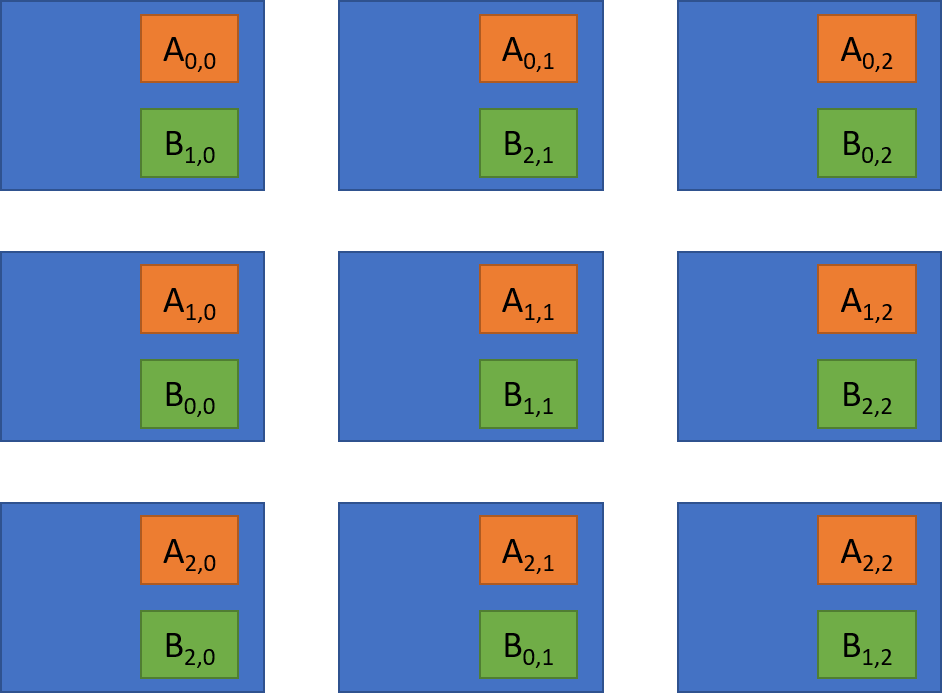
\includegraphics[width=1.0\textwidth]{step_0_cannon}
	\end{columns}
\end{frame}
%=============================================
\begin{frame}
\frametitle{HPX : High Performance Parallex}
\begin{block}{A C++ runtime system for applications of any scale \footnote{\tiny\textit
{Parallex an advanced parallel execution model for scaling-impaired applications}-
H. Kaiser et al - ICPPW, 2009}$^{,}$\footnote{\tiny\textit{A Task Based Programming Model in
a Global Address Space} - H. Kaiser et al - PGAS, 2014\newline}}
    \begin{itemize}
    \item
    \item
    \item
    \end{itemize}
\end{block}
\begin{block}{Subtitle 2}
    \begin{itemize}
    \item
    \item
    \item
    \end{itemize}
\end{block}
\end{frame}
%====================================================
\begin{frame}
\frametitle{Example code}
\begin{block}{C++ code}
    \vspace{0.3cm}
    \cppexample
\end{block}
\end{frame}
%====================================================
\begin{frame}
\begin{center}\LARGE Thanks for your attention\end{center}
\end{frame}
%=============================================
\end{document}
